\section{Funktionen und Stetigkeit}

\subsection{Eigenschaften von Funktionen}

\begin{definition}{Umkehrfunktion}
    Eine bijektive Funktion $f: D \rightarrow W$ besitzt eine Umkehrfunktion $f^{-1}: W \rightarrow D$.

    \textbf{Vorgehen zum Bestimmen von $f^{-1}$ aus $f(x)=y$:}
    \begin{enumerate}
        \item Nach $x$ auflösen: $x=g(y)$
        \item Variablen vertauschen: $y=g(x)$
    \end{enumerate}
\end{definition}

\begin{theorem}{Operationen von Funktionen}
    Seien $f, g: D \to \R$ zwei Funktionen. Dann sind definiert:
    \begin{itemize}
        \item Addition: $x \rightarrow f(x)+g(x)$
        \item Subtraktion: $x \rightarrow f(x)-g(x)$
        \item Multiplikation: $x \rightarrow f(x) \cdot g(x)$
        \item Division: $x \rightarrow f(x) / g(x)$ (falls $g(x) \neq 0$)
        \item Komposition/Verkettung: $(g \circ f)(x)=g(f(x))$
    \end{itemize}
\end{theorem}

\begin{definition}{Symmetrie}
    Eine Funktion $f: D \to \R$ heisst:
    \begin{itemize}
        \item \textbf{gerade}, falls $f(-x)=f(x)$ für alle $x \in D$
        \item \textbf{ungerade}, falls $f(-x)=-f(x)$ für alle $x \in D$
    \end{itemize}
\end{definition}

\begin{center}
    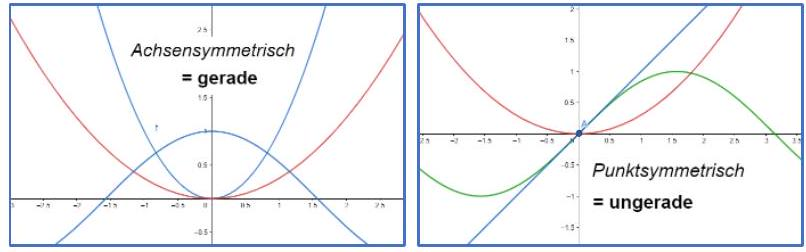
\includegraphics[scale=0.3]{2024_01_20_7bfda6c084929ccc01ffg-01(2).jpg}
\end{center}

\begin{definition}{Beschränktheit}
    Sei $f \in \R^D$.
    \begin{enumerate}
        \item $f$ ist \emph{nach oben beschränkt}, falls $f(D) \subseteq \R$ nach oben beschränkt ist.
        \item $f$ ist \emph{nach unten beschränkt}, falls $f(D) \subseteq \R$ nach unten beschränkt ist.
        \item $f$ ist \emph{beschränkt}, falls $f(D) \subseteq \R$ beschränkt ist.
    \end{enumerate}
\end{definition}

\begin{definition}{Monotonie}
    Eine Funktion $f: D \to \R$ heisst für $x_1, x_2 \in D$ mit $x_1 < x_2$:
    \begin{itemize}
        \item \textbf{monoton wachsend}, falls $f(x_1) \leq f(x_2)$
        \item \textbf{streng monoton wachsend}, falls $f(x_1) < f(x_2)$
        \item \textbf{monoton fallend}, falls $f(x_1) \geq f(x_2)$
        \item \textbf{streng monoton fallend}, falls $f(x_1) > f(x_2)$
    \end{itemize}
\end{definition}

\subsection{Stetigkeit}

\begin{definition}{Stetigkeit}
    Eine Funktion ist stetig, falls:
    \begin{itemize}
        \item die Kurve keine Sprünge macht
        \item man den Graphen der Funktion zeichnen kann, ohne den Stift dabei abzusetzen
    \end{itemize}
\end{definition}

\begin{formula}{Spezielle Stetige Funktionen}
    \begin{enumerate}
        \item $|f|$, $\max(f, g)$ und $\min(f, g)$ sind stetig, falls $f$ und $g$ stetig sind
        \item Polynomielle Funktionen sind auf ganz $\R$ stetig
        \item Die trigonometrischen Funktionen $\sin : \R \to \R$ und $\cos : \R \to \R$ sind stetig
        \item Die Exponentialfunktion $e^x$ ist auf ganz $\R$ stetig
    \end{enumerate}
\end{formula}

\begin{center}
    \begin{tikzpicture}[state/.style={draw, text width = 30mm, align = center, rounded corners = 3pt}]
        \node[state] (ls) {$f$ Lipschitz stetig};
        \node[state, below = 4mm of ls, blue, thick, text = black] (gs) {$f$ gleichmässig stetig};
        \node[state, right = 4mm of gs] (diff) {$f$ differenzierbar};
        \node[state, below = 4mm of gs, blue, thick, text = black] (s) {$f$ stetig};

        \draw[->] (diff) |- (ls) node[midway, above] {Ableitung beschränkt};
        \draw[->] (ls) -- (gs);
        \draw[->, blue, thick] (gs) -- (s);
        \draw[->] (s.west) -- ($(s.west) - (0.25, 0)$) |- (gs) node[pos = 0.25, left] {$\Omega$ kompakt};
    \end{tikzpicture}
\end{center}

\subsection{Grenzwerte von Funktionen}

\begin{highlight}{Wichtige Grenzwerte}
    \begin{center}
        \begin{minipage}{0.4\linewidth}
            \tcbsubtitle{Harmonische Folge:}
            $$\lim_{n \rightarrow \infty} \frac{1}{n}=0$$
            \tcbsubtitle{Geometrische Folge:}
            $$\lim_{n \rightarrow \infty} q^n=0 \quad(|q|<1)$$
        \end{minipage}
        \hfill\vline\hfill
        \begin{minipage}{0.5\linewidth}
            \tcbsubtitle{n-te Wurzel:}
            $$\lim_{n \rightarrow \infty} \sqrt[n]{a}=1$$
            \tcbsubtitle{Eulerzahl:}
            $$\lim_{n \rightarrow \infty}\left(1+\frac{1}{n}\right)^n=e$$
        \end{minipage}
    \end{center}
\end{highlight}

\begin{definition}{Konvergenz einer Funktion}
    Die Funktion $y = f(x)$ hat an der Stelle $x_0$ den Grenzwert $y_0$, falls:

    für jede Folge $(x_n)$ mit $\lim_{n \rightarrow \infty} x_n=x_0$ gilt $\lim_{n \rightarrow \infty} f(x_n)=y_0$.

    \textbf{Bemerkung:} Die Stelle $x_0$ muss nicht im Definitionsbereich $D$ liegen.
\end{definition}

\begin{definition}{Konvergenz und Divergenz}
    \begin{itemize}
        \item \textbf{Konvergenz:} Funktion mit Grenzwert für $x \rightarrow \infty$
        \item \textbf{Divergenz:} Funktion ohne Grenzwert für $x \rightarrow \infty$
        \item \textbf{Bestimmte Divergenz:} Funktion mit $\lim_{x \rightarrow \infty} f(x)= \pm \infty$
    \end{itemize}
\end{definition}

\begin{definition}{Links- und Rechtsseitige Grenzwerte}
    Sei $f : D \to \R$ und $x_0 \in \R$ ein Häufungspunkt. Das bedeutet vereinfacht, dass die Funktion an dieser Stelle evtl. einen Sprung macht, da sich z.B. die Definition ändert.

    \textbf{Beispiel:}
    \begin{equation*}
        f(x) = \begin{cases}
            0 & x < 0\\
            1 & x \geq 0
        \end{cases}
    \end{equation*}

    Setze in diesem Beispiel $x_0 = 0$ und prüfe, ob sich die Funktion von rechts und links dem selben Wert nähert bei $x_0$. (NEIN in diesem Beispiel.)

    \textbf{Formell:} Eine Funktion ist gleichmässig konvergent, wenn für alle Werte gilt:
    $$\lim_{x \to x_0^+} f(x) = \lim_{x \to x_0^-} f(x)$$
    (Linksseitiger Grenzwert = Rechtsseitiger Grenzwert)
\end{definition}

\begin{example2}{Grenzwert einer Funktion}
    Betrachte $f(x)=\frac{x^2-1}{x-1}$ an der Stelle $x_0=1$:

    \begin{center}
        \begin{tabular}{|c|c|c|}
            \hline
            $n$ & $x_n=1-\frac{1}{n}$ & $f(x_n)$ \\
            \hline
            $1$ & 0 & 1 \\
            \hline
            $2$ & 0.5 & 1.5 \\
            \hline
            $3$ & 0.66 & 1.66 \\
            \hline
            $4$ & 0.75 & 1.75 \\
            \hline
            $5$ & 0.8 & 1.8 \\
            \hline
            $10$ & 0.9 & 1.9 \\
            \hline
            $100$ & 0.99 & 1.99 \\
            \hline
            $1000$ & 0.999 & 1.999 \\
            \hline
            $n \rightarrow \infty$ & $x_0=1$ & 2 \\
            \hline
        \end{tabular}
    \end{center}

    Somit gilt: $\lim_{x \rightarrow 1} f(x)=2$
\end{example2}

\subsubsection{Rechnen mit Grenzwerten}

\begin{corollary}{Rechnen mit Grenzwerten von Funktionen}
    Seien $f, g: D \to \R$ Funktionen und existieren die entsprechenden Grenzwerte, dann gilt:
    \begin{itemize}
        \item $\lim_{x \to x_0} (f + g)(x) = \lim_{x \to x_0} f(x) + \lim_{x \to x_0} g(x)$
        \item $\lim_{x \to x_0} (f \cdot g)(x) = \lim_{x \to x_0} f(x) \cdot \lim_{x \to x_0} g(x)$
        \item Sei $f \leq g$, so ist $\lim_{x \to x_0} f(x) \leq \lim_{x \to x_0} g(x)$
        \item Falls $g_1 \leq f \leq g_2$ und $\lim_{x \to x_0} g_1(x) = \lim_{x \to x_0} g_2(x)$, so existiert $\lim_{x \to x_0} f(x) = \lim_{x \to x_0} g_1(x)$
    \end{itemize}
\end{corollary}

\begin{concept}{l'Hospital Regel}
    Seien $f,g : ]a,b[ \to \R$ differenzierbar mit $g'(x) \neq 0$ für alle $x \in ]a,b[$.

    Falls $\lim_{x \to b^-} f(x) = 0$, $\lim_{x \to b^-} g(x) = 0$ und $\lambda \coloneqq \lim_{x \to b^-} \frac{f'(x)}{g'(x)}$ existiert, folgt:
    \begin{iequation}
        \lim_{x \to b^-} \frac{f(x)}{g(x)} = \lim_{x \to b^-}\frac{f'(x)}{g'(x)}
    \end{iequation}
    \tcblower
    \emph{Nur für $\lim_{x \to 0} \frac{f(x)}{g(x)} = \frac{\text{``}0\text{''}}{  \text{``}0\text{''}}$ oder $\frac{\text{``}\infty\text{''}}{\text{``}\infty\text{''}}$ erlaubt.}
\end{concept}

\subsubsection{Strategien und Rechentricks}

\begin{KR}{Erweitern mit $\left(\frac{1}{n^k}\right)$}
    $k=$ höchste Potenz
\end{KR}

\begin{example}
    Beispiel:
    $$
    \begin{aligned}
        \lim_{n \rightarrow \infty} \frac{3 n^2+2 n+1}{5 n^2+4 n+2}
        &\Longrightarrow \textcolor{pink}{\frac{\frac{1}{n^2}}{\frac{1}{n^2}}} \cdot \frac{3 n^2+2 n+1}{5 n^2+4 n+2} \\
        &= \frac{\frac{3 n^2}{n^2}+\frac{2 n}{n^2}+\frac{1}{n^2}}{\frac{5 n^2}{n^2}+\frac{4 n}{n^2}+\frac{2}{n^2}} \\
        &= \frac{3+\frac{2}{n}+\frac{1}{n^2}}{5+\frac{4}{n}+\frac{2}{n^2}}
        = \frac{3+0+0}{5+0+0} = \frac{3}{5}
    \end{aligned}
    $$
\end{example}

\begin{KR}{Erweitern mit $\left(\frac{1}{a^k}\right)$}
    $k=$ höchste Potenz, $a=$ grösste Basis
\end{KR}

\begin{example}
    Beispiel:
    $$
    \begin{aligned}
        \lim_{n \rightarrow \infty} \frac{3^{n+1}+2^n}{3^n+2}
        &\Longrightarrow \textcolor{pink}{\frac{\frac{1}{3^n}}{\frac{1}{3^n}}} \cdot \frac{3 \cdot 3^n+2^n}{3^n+2} \\
        &= \frac{\frac{3 \cdot 3^n}{3^n}+\frac{2^n}{3^n}}{\frac{3^n}{3^n}+\frac{2}{3^n}} \\
        &= \frac{3+\frac{2^n}{3^n}}{1+\frac{2}{3^n}}
        = \frac{3+0}{1+0} = 3
    \end{aligned}
    $$
\end{example}

\begin{KR}{Erweitern mit $\sqrt{a(n)}+\sqrt{b(n)}$}
    Nützlich bei Differenzen von Wurzeln
\end{KR}

\begin{example}
    Beispiel:
    $$
    \begin{aligned}
        &\lim_{n \rightarrow \infty} \sqrt{n^2+n}-\sqrt{n^2-2 n}\\
        &\Longrightarrow \textcolor{pink}{\frac{\sqrt{n^2+n}+\sqrt{n^2-2 n}}{\sqrt{n^2+n}+\sqrt{n^2-2 n}}} \cdot \frac{\sqrt{n^2+n}-\sqrt{n^2-2 n}}{1} \\
        &= \frac{(n^2+n)-(n^2-2 n)}{\sqrt{n^2+n}+\sqrt{n^2-2 n}}
        = \frac{3 n}{\sqrt{n^2+n}+\sqrt{n^2-2 n}}\\
        &= \frac{\frac{1}{n}}{\frac{1}{n}} \cdot \frac{3 n}{\sqrt{n^2+n}+\sqrt{n^2-2 n}} \\
        &= \frac{\frac{3 n}{n}}{\sqrt{\frac{n^2+n}{n^2}}+\sqrt{\frac{n^2-2 n}{n^2}}}
        = \frac{3}{\sqrt{1+\frac{1}{n}}+\sqrt{1-\frac{2}{n}}} \\
        &= \frac{3}{\sqrt{1}+\sqrt{1}} = \frac{3}{2}
    \end{aligned}
    $$
\end{example}

\begin{KR}{Erweitern zur Eulerzahl}
    Forme um zu $\lim_{x \rightarrow \infty}\left(\left(1+\frac{1}{x}\right)^{x}\right)^{a}=e^{a}$
\end{KR}

\begin{example}
    Beispiel:
    $$
    \begin{aligned}
        &\lim_{n \rightarrow \infty}\left(1+\frac{2}{3 n}\right)^{4 n}
        = \left(\left(1+\frac{1}{\frac{3 n}{2}}\right)^{\frac{3 n}{2}}\right)^{a}=e^{a}=e^{\frac{8}{3}}\\
        &\text{Wir rechnen also:}\\
        &4 n=\frac{3 n}{2} \cdot a \text{ und } a=\frac{4 n}{\frac{3 n}{2}}=\frac{8}{3}
    \end{aligned}
    $$
\end{example}

\subsection{Spezielle Sätze}

\begin{definition}{Kompaktes Intervall}
    Ein Intervall $I \subseteq \R$ ist kompakt, falls es von der Form $I=[a,b]$ mit $a \leq b$ ist.
\end{definition}

\textbf{Bemerkung:} Für $x_0$ in einem kompakten Intervall gibt es immer mindestens eine Folge $(a_n)_{n\geq 1}$ mit $a_n \in I$, so dass $\lim_{n \to \infty} a_n = x_0$.

\begin{lemma}{Min-Max Satz}
    Sei $(x_n)$ eine konvergente Folge in $\R$ mit Grenzwert $\lim_{n \to \infty} x_n \in \R$. Sei $a \leq b$. Falls $\{x_n : n \geq 1\} \subseteq [a,b]$, folgt $\lim_{n \to \infty} x_n \in [a,b]$.
\end{lemma}

\begin{theorem}{Minimum-Maximum-Theorem}
    Sei $f:I= [a,b] \to \R$ stetig auf einem kompakten Intervall $I$. Dann gibt es $u \in I$ und $v \in I$ mit:
    \begin{equation*}
        f(u) \leq f(x) \leq f(v) \qquad \forall x \in I
    \end{equation*}
    Insbesondere ist $f$ beschränkt und nimmt ihr Minimum in $u$ und ihr Maximum in $v$ an.
\end{theorem}

\textbf{Zusammen mit dem Zwischenwertsatz folgt:} $f([a,b]) = [f(u), f(v)]$

\begin{lemma}{Zwischenwertsatz}
    Sei $I \subseteq \R$ ein Intervall, $f: I \to \R$ eine stetige Funktion und $a,b \in I$.

    Für jedes $c$ zwischen $f(a)$ und $f(b)$ gibt es ein $z$ zwischen $a$ und $b$ mit $f(z) = c$.
\end{lemma}

\textbf{Bemerkung:} Der Zwischenwertsatz wird oftmals verwendet, um zu zeigen, dass eine Funktion einen gewissen Wert annimmt.

\begin{KR}{Anwendung: Nullstellen}
    \begin{enumerate}
        \item Sei $f:[a,b] \to \R$ stetig. Falls $f(a) \cdot f(b) < 0$, dann $\exists c \in ]a,b[$ mit $f(c) = 0$ (Also eine Nullstelle)
        \item Sei $P(x) = a_n x^n + a_{n-1}x^{n-1} + \ldots + a_0$ ein Polynom mit $a_n \neq 0$ und $n$ ungerade. Dann besitzt $P$ mindestens eine Nullstelle in $\R$
    \end{enumerate}
\end{KR}

\textbf{Gegenbeispiel:} Für $c > 0$ besitzt $Q(x) = x^2 + c$ keine Nullstelle in $\R$.

\begin{center}
    \begin{minipage}{0.44\linewidth}
        Falls eine Funktion wie abgebildet springt, lässt sich der Zwischenwertsatz nicht anwenden.
    \end{minipage}
    \hfill
    \begin{minipage}{0.25\linewidth}
        \begin{equation*}
            f(x) = \begin{cases}
                0 & x < 0\\
                1 & x \geq 0
            \end{cases}
        \end{equation*}
    \end{minipage}
    \hfill
    \begin{minipage}{0.25\linewidth}
        \begin{center}
            \begin{tikzpicture}
                \begin{axis}[
                    axis x line = middle,
                    axis y line = none,
                    ytick style={draw=none},
                    yticklabels={,,},
                    xtick style={draw=none},
                    xticklabels={,,},
                    width = 30mm,
                    ticklabel style = {font=\tiny},
                    ymin = -0.2,
                    ymax = 0.9,
                    xmin = -2,
                    xmax = 2
                ]
                    \filldraw[darkblue] (axis cs: 0,0.75) circle (0.5pt);
                    \addplot[thick, darkblue, ->] coordinates {(-2,0) (0,0)};
                    \addplot[thick, darkblue, ->] coordinates {(0,0.75) (2,0.75)};
                    \begin{pgfonlayer}{bg}
                        \fill[green!30, rounded corners = 1pt] (axis cs: -0.2, 0.85) rectangle (axis cs: 0.2, -0.1);
                    \end{pgfonlayer}
                \end{axis}
            \end{tikzpicture}
        \end{center}
    \end{minipage}
\end{center}

\subsection{Umkehrabbildungen}

\begin{lemma}{Satz über die Umkehrabbildung}
    Sei $I \subseteq \R$ ein Intervall und $f:I \to \R$ stetig und streng monoton.

    Dann ist $J \coloneqq f(I) \subseteq \R$ ein Intervall und $f^{-1}: J \to I$ ist stetig und streng monoton.
\end{lemma}

\begin{center}
    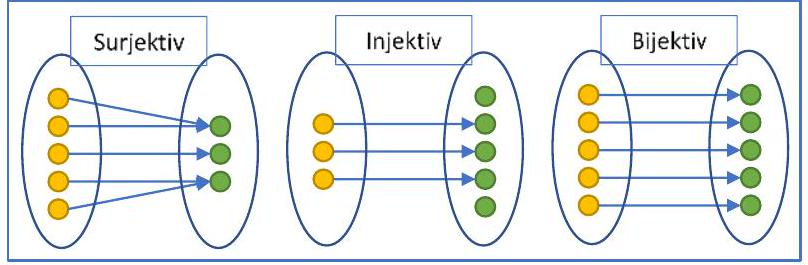
\includegraphics[scale=0.2]{2024_01_20_7bfda6c084929ccc01ffg-01(3).jpg}
\end{center}

\begin{example}
    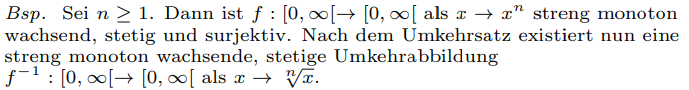
\includegraphics[scale=0.5]{bsp_umkehrabbildung.png}
\end{example}

\subsection{Funktionenfolgen und Funktionenreihen}

Analog zur Folge definieren wir die (reellwertige) \textit{Funktionenfolge} als eine Abbildung $\N \to \R^D$, $n \mapsto f_n$.

Wir bezeichnen $f(n)$ als $f_n$ (n-te Folge) und die Funktionenfolge mit $(f_n)_{n\geq 0}$.

Für jedes $x \in D$ erhält man eine Folge $(f_n(x))_{n \geq 0}$ in $\R$ (wobei $D$ eine Menge ist).

\begin{definition}{Punktweise Konvergenz}
    Die Funktionenfolge $(f_n)_{n\geq 0}$ \emph{konvergiert punktweise} gegen die Funktion $f:D \to \R$, falls für alle $x \in D$ gilt:
    $$f(x) = \lim_{n \to \infty} f_n(x)$$
\end{definition}

\textbf{Warnung:} Nur weil eine Funktionenfolge $(f_n)_{n\geq 0}$ aus stetigen Funktionen besteht, ist die Grenzfunktion $f$ nicht unbedingt stetig.

\begin{definition}{Gleichmässige Konvergenz ($\varepsilon$-Definition)}
    Die Folge $f_n : D \to \R$ \emph{konvergiert gleichmässig} in $D$ gegen $f: D \to \R$, falls gilt:

    $\forall \varepsilon > 0~\exists N \geq 1$, sodass
    \begin{equation*}
        \forall n \geq N, \forall x \in D: |f_n(x) - f(x)| < \varepsilon
    \end{equation*}

    Für Funktionenfolgen: $\forall n,m \geq N$ und $\forall x \in D: |f_n(x) - f_m(x)| < \varepsilon$
\end{definition}

\begin{theorem}{Konvergenz und Stetigkeit}
    Sei $D \subseteq \R$ und $(f_n)_{n\geq 0}$ eine Funktionenfolge aus (in $D$) stetigen Funktionen, die (in $D$) gleichmässig gegen die Funktion $f:D \to \R$ konvergiert.

    Dann ist $f$ (in $D$) stetig.
\end{theorem}

\begin{definition}{Gleichmässige Konvergenz (Limes-Definition)}
    Eine Funktionenfolge $f_n : D \to \R$ ist \emph{gleichmässig konvergent}, falls für alle $x \in D$ der Grenzwert $f(x) \coloneqq \lim_{n \to \infty} f_n(x)$ existiert und die Folge $(f_n)_{n\geq 0}$ gleichmässig gegen $f$ konvergiert.

    Falls $f_n$ eine gleichmässig konvergente Folge stetiger Funktionen ist, dann ist die Funktion $f(x) \coloneqq \lim_{n \to \infty} f_n(x)$ stetig.
\end{definition}

\begin{definition}{Konvergenz von Funktionenreihen}
    Die Reihe $\sum_{k=0}^\infty f_k(x)$ konvergiert gleichmässig (in $D$), falls die durch
    $$S_n(x) \coloneqq \sum_{k=0}^n f_k(x)$$
    definierte Funktionenfolge gleichmässig konvergiert und deren Grenzwert
    $$f(x) \coloneqq \sum_{k=0}^\infty f_k(x)$$
    eine stetige Funktion ist.
\end{definition}

\begin{theorem}{Gleichmässige Konvergenz und Stetigkeit}
    Sei $\sum_{k=0}^\infty c_k x^k$ eine Potenzreihe mit positivem Konvergenzradius $\rho > 0$ und sei:
    \begin{equation*}
        f(x) \coloneqq \sum_{k=0}^\infty c_k x^k \qquad |x| < \rho
    \end{equation*}

    Dann gilt: $\forall 0 \leq r < \rho$ konvergiert $\sum_{k=0}^\infty c_k x^k$ gleichmässig auf $[-r,r]$.

    Insbesondere ist $f:]-\rho, \rho[ \to \R$ stetig. Absolut konvergente Potenzreihen sind stetig.
\end{theorem}

\begin{KR}{Strategie: Konvergenz von Funktionenfolgen}
    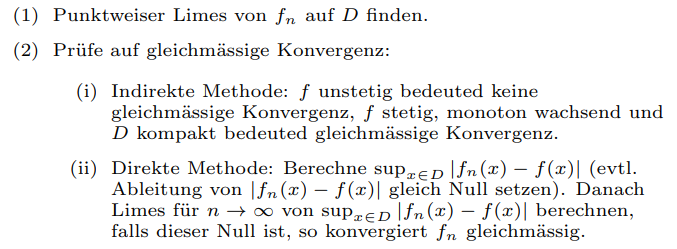
\includegraphics[scale=0.5]{strategie_konvergenz_funktionenfolgen.png}
\end{KR}

\subsection{Konvergenzradius}

\subsubsection{Potenzreihe und Konvergenzradius}

\begin{definition}{Potenzreihe}
    Eine Potenzreihe ist eine Reihe von der Form $\sum_{k=0}^\infty c_k z^k$, wobei $(c_k)_{k\geq 0}$ eine Folge ist.
\end{definition}

\begin{corollary}{Konvergenz und Divergenz}
    Die Potenzreihe $\sum_{k=0}^\infty c_k z^k$ konvergiert absolut für alle $|z| < \rho$ und divergiert für alle $|z| > \rho$.
\end{corollary}

Der Konvergenzradius ($\rho$) gibt an, in welchem Bereich von $\R$ bzw. $\C$ die Konvergenz garantiert ist. Die Potenzreihe hat \emph{positiven Konvergenzradius}, falls $\limsup_{k \to \infty} \sqrt[k]{|c_k|}$ existiert.

Der Konvergenzradius ist dann definiert als:
\begin{equation*}
    \rho = \begin{cases}
        + \infty & \text{falls}~\limsup_{k \to \infty} \sqrt[k]{|c_k|} = 0\\
        \frac{1}{\limsup_{k \to \infty} \sqrt[k]{|c_k|}} & \text{falls}~\limsup_{k \to \infty} \sqrt[k]{|c_k|} > 0
    \end{cases}
\end{equation*}

Alternativ lässt sich der Konvergenzradius auch mit $\rho = \lim_{n \to \infty} \left| \frac{a_n}{a_{n+1}} \right|$ berechnen.
